% Created 2018-10-05 Fri 01:01
% Intended LaTeX compiler: pdflatex
\documentclass[10pt,t]{beamer}
\usepackage[utf8]{inputenc}
\usepackage[T1]{fontenc}
\usepackage{graphicx}
\usepackage{grffile}
\usepackage{longtable}
\usepackage{wrapfig}
\usepackage{rotating}
\usepackage[normalem]{ulem}
\usepackage{amsmath}
\usepackage{textcomp}
\usepackage{amssymb}
\usepackage{capt-of}
\usepackage{hyperref}
\usetheme{default}
\author{L. Larrabee Strow}
\date{\today}
\title{\large Can We Improve the AIRS ILS Functions Using CrIS?}
\date{\textit{\footnotesize June 20, 2018}}
\input beamer_setup
\usetheme{metropolis}
\metroset{titleformat title=allcaps}
\renewcommand{\UrlFont}{\small\tt}
\renewcommand*{\UrlFont}{\footnotesize}
\tolerance=1000
\RequirePackage{fancyvrb}
\DefineVerbatimEnvironment{verbatim}{Verbatim}{fontsize=\footnotesize}
\author{L.~Larrabee~Strow, Howard~Motteler, Chris~Hepplewhite, Steven  ~Buczkowski, and Sergio~De-Souza~ Machado (UMBC)}
\hypersetup{
 pdfauthor={L. Larrabee Strow},
 pdftitle={\large Can We Improve the AIRS ILS Functions Using CrIS?},
 pdfkeywords={},
 pdfsubject={},
 pdfcreator={Emacs 25.1.1 (Org mode 9.1.12)}, 
 pdflang={English}}
\begin{document}

\maketitle
\addtobeamertemplate{block begin}{
  \setlength{\parsep}{0pt}
  \setlength{\topsep}{3pt plus 2pt minus 2.5pt}
  \setlength{\itemsep}{0pt plus 0pt minus 2pt}
  \setlength{\partopsep}{2pt}
}

\begin{frame}[label={sec:orga895e5d}]{AIRS SNOs with IASI and CrIS Show Same Patterns}
\vspace{-0.1in}
\begin{itemize}
\item SNO differences are run through a high-pass only filter
\item Eliminates smooth SNO diffs that could be CrIS, IASI, or AIRS
\end{itemize}

\begin{center}
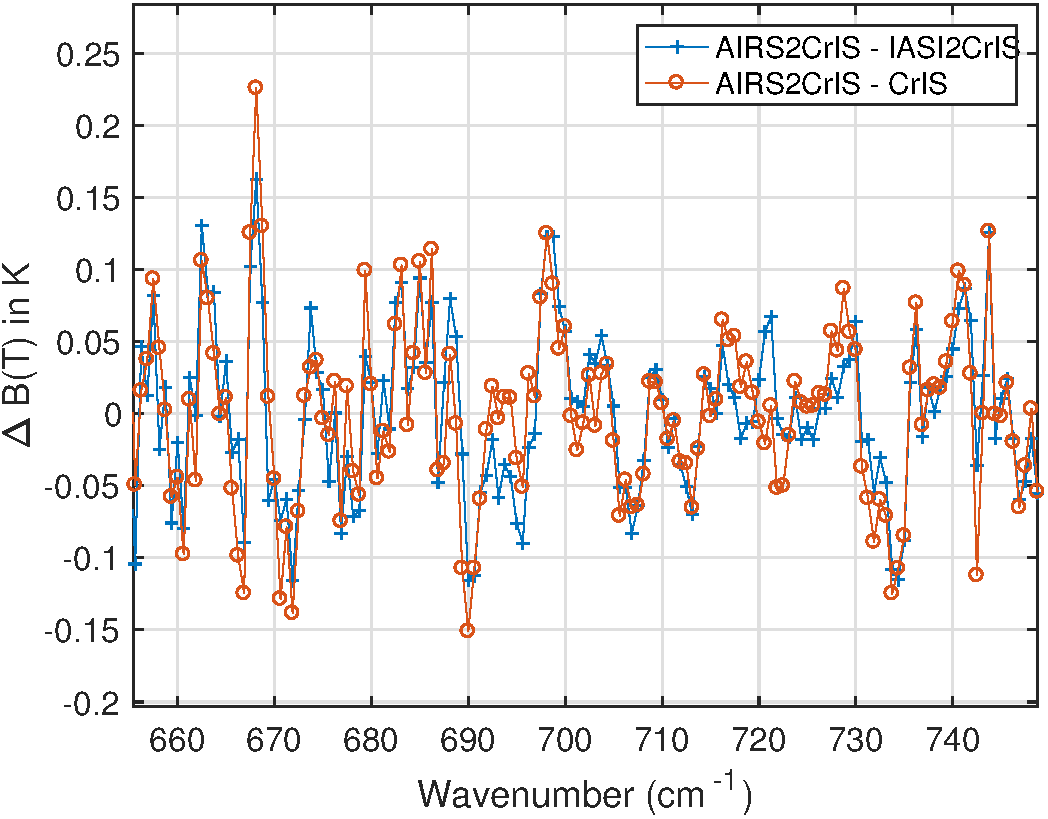
\includegraphics[width=0.75\linewidth]{./wFigs/good_a2c_same_cris_or_iasi.pdf}
\end{center}
\end{frame}

\begin{frame}[label={sec:orgdfdb9ea}]{Could Patterns be due to AIRS SRF Width Errors?}
\vspace{-0.1in}
\begin{itemize}
\item AIRS SRF width uncertainties are \textasciitilde{}5\% (TVAC data)
\item Black line: reduce SRFs by 5\%, what is the expected SNO difference
\end{itemize}

\begin{center}
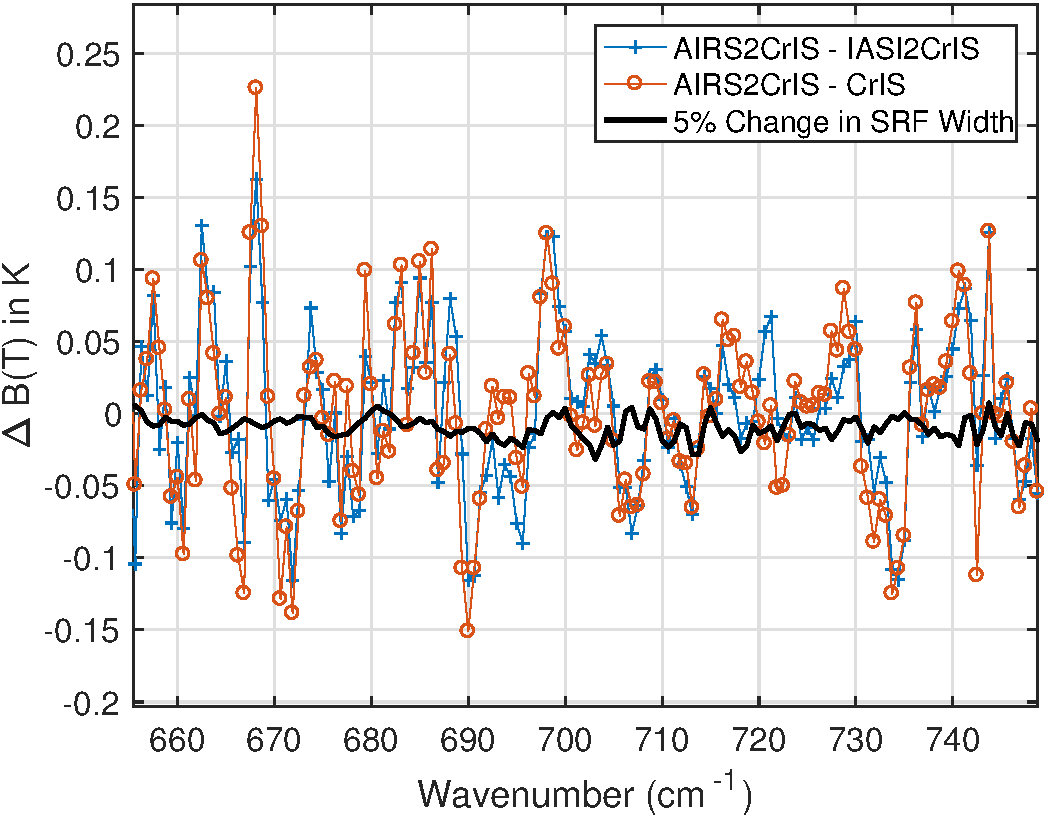
\includegraphics[width=0.75\linewidth]{./wFigs/good_a2c_same_cris_or_iasi_sim_5pc_lowered_width.pdf}
\end{center}
\end{frame}

\begin{frame}[shrink=10,label={sec:org97f1f2a}]{Other SRF Errors, since it is not the widths?}
\vspace{-0.1in}
\begin{itemize}
\item Simulations of SNO sensitivty to uncertainties in the SRF \emph{centroids} are too small to create observed patterns

\item Entrance filter fringe shifts (seen before/after Nov. 2003 Aqua shutdown) are not the cause, they are far too small
\end{itemize}

Tom Pagano has done a re-calibration of AIRS L1b based on a better analysis of TVAC data.  The new candidate calibration is v7 (as opposed to present v5 calibration)

\vspace{0.1in}

We now compare the SNO data to the v5 - v7 calibration differences.

We show two types of plots:
\begin{enumerate}
\item AIRS/CrIS SNOs compared to V5 - V7 calibration differences
\item AIRS/CrIS v5 SNOs (present L1b) compared to AIRS/CrIS v7 SNOs
\end{enumerate}

\vspace{0.1in}

AIRS/CrIS v7 SNOs = (AIRS\_v5/CrIS SNOs) - (v5 - v7 Cal Diffs)
\end{frame}

\begin{frame}[label={sec:orgbff59a0}]{First Convert v5 - v7 B(T) Differences to CrIS ILS/SRF}
\vspace{-0.3in}

\begin{columns}
\begin{column}{0.55\columnwidth}
\begin{block}{}
\begin{center}
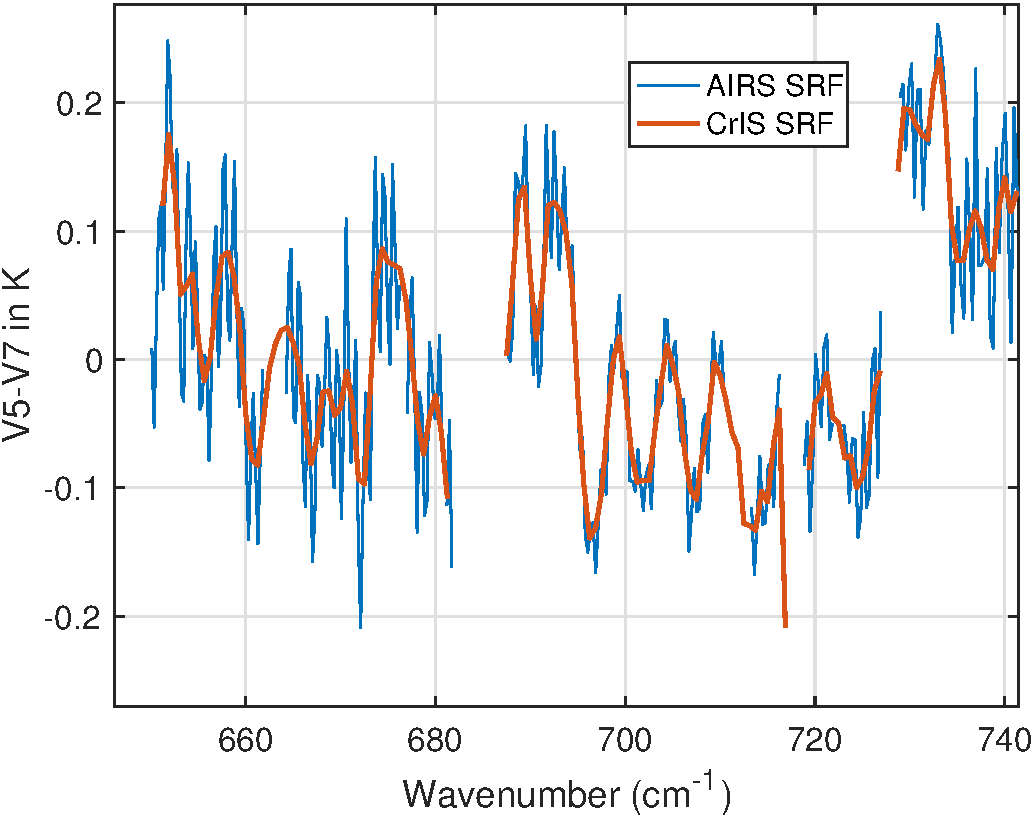
\includegraphics[width=\linewidth]{./Figs/Pdf/v5_minus_v7_airs_srf_and_airs2cris_lw_only.pdf}
\end{center}
\end{block}
\end{column}

\begin{column}{0.55\columnwidth}
\begin{block}{Approach}
\vspace{-0.1in}
\begin{itemize}
\item Tom Pagano's v5 - v7 differences use AIRS SRF, 2378 channel set
\item We need to compare to CrIS on the AIRS2CrIS scale (CrIS NSR resolution)
\item Conversion to CrIS SRF
\begin{enumerate}
\item We add Tom's v5 - v7 to a similar L1c B(T) spectrum
\item Convert this to AIRS2CrIS
\item Subtract this B(T) from un-perturbed AIRS2CrIS spectrum
\item You now have Tom's v5-v7 diffs on the CrIS SRF scale
\end{enumerate}
\end{itemize}
\end{block}
\end{column}
\end{columns}
\end{frame}


\begin{frame}[label={sec:orgc33581c}]{Overview of SNO Diffs to v5-v7 Diffs}
\vspace{-0.1in}
\begin{center}
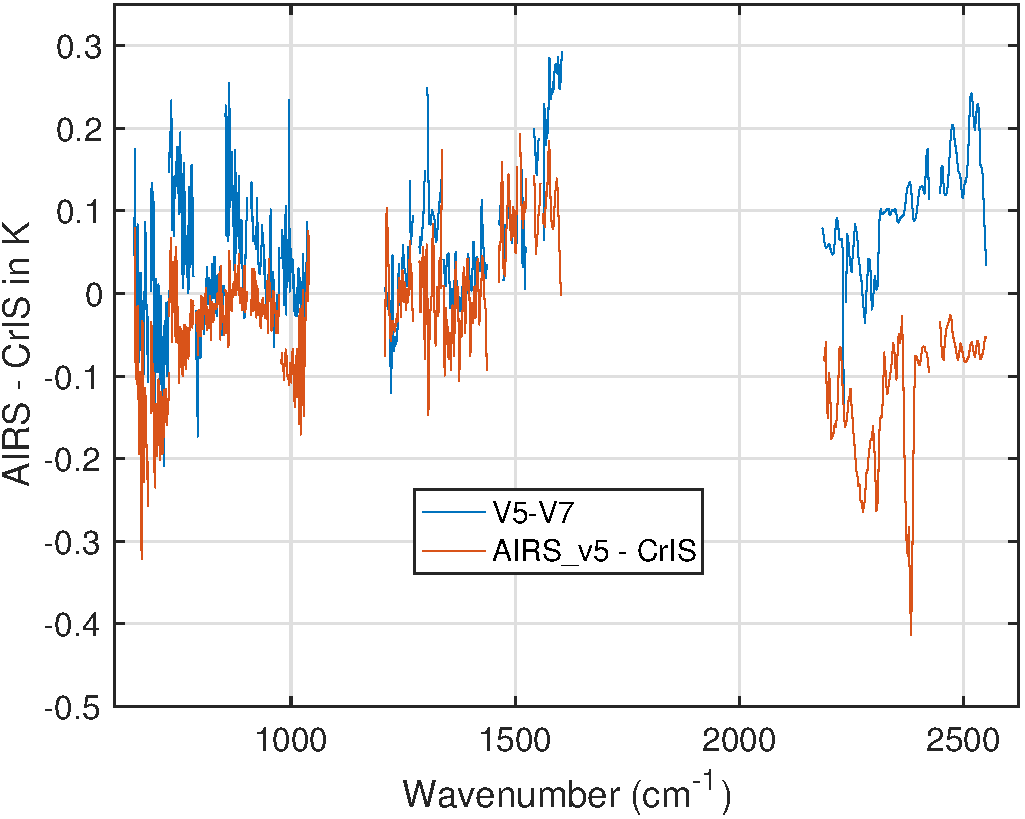
\includegraphics[width=0.75\linewidth]{./Figs/Pdf/airs_v5_sno_minus_cris_and_v5_minus_v7.pdf}
\end{center}

\vspace{-0.1in}
\begin{itemize}
\item Highest similarity in the mid-wave
\item Same similar patterns in the long-wave
\end{itemize}
\end{frame}

\begin{frame}[label={sec:org6b8d527}]{Create SNO\_v7 and Compare to SNO\_v5}
\vspace{-0.1in}
\begin{center}
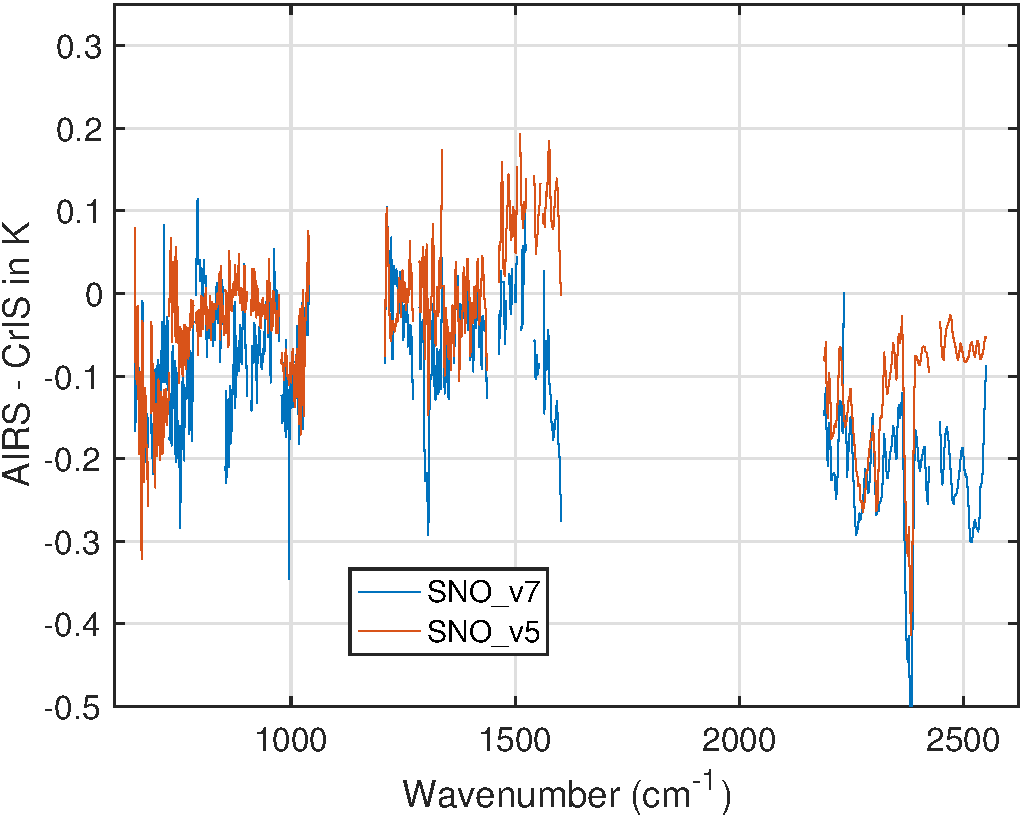
\includegraphics[width=0.75\linewidth]{./Figs/Pdf/airs_v7_sno_and_airs_v5_sno.pdf}
\end{center}

\vspace{-0.1in}
\begin{itemize}
\item Shortwave: v5 SNO "better", ie smaller SNO differences
\end{itemize}
\end{frame}

\begin{frame}[label={sec:orgd0928c9}]{Midwave SNO\_v7 versus SNO\_v5}
\vspace{-0.1in}
\begin{center}
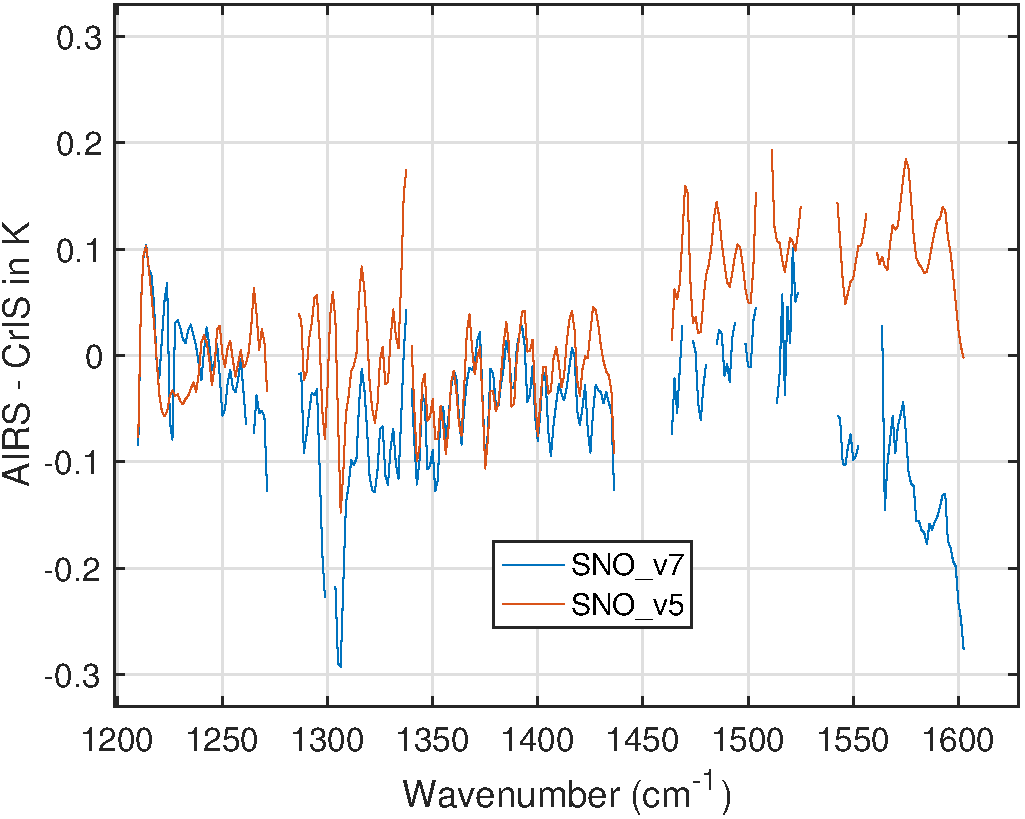
\includegraphics[width=0.75\linewidth]{./Figs/Pdf/airs_v7_sno_and_airs_v5_sno_mw.pdf}
\end{center}

\vspace{-0.1in}
\begin{itemize}
\item v7 Problems near 1300 \wn (low B(T)'s there)
\item Some improvement with v7 near 1500 \wn, but no obvious winner
\end{itemize}
\end{frame}

\begin{frame}[label={sec:orgdddbacb}]{Longwave SNO\_v7 versus SNO\_v5}
\vspace{-0.1in}
\begin{center}
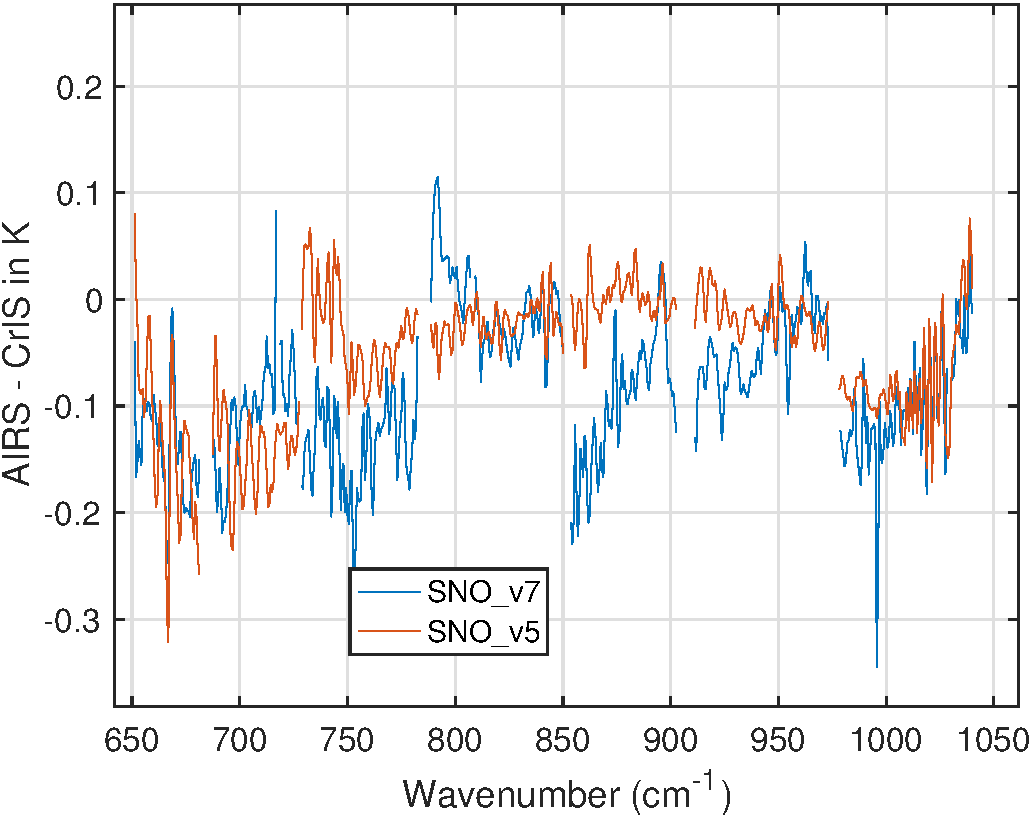
\includegraphics[width=0.75\linewidth]{./Figs/Pdf/airs_v7_sno_and_airs_v5_sno_lw.pdf}
\end{center}

\vspace{-0.1in}
\begin{itemize}
\item SNO\_v5 more uniform
\end{itemize}
\end{frame}


\begin{frame}[label={sec:orgee82d00}]{Conclusions}
\begin{itemize}
\item Both AIRS-CrIS and AIRS-IASI SNOs suggest that AIRS radiances have significant channel-to-channel calibration differences
\item We cannot attribute those differences to the AIRS SRF wdiths, centroid, or entrance filter fringe shifts
\item Tom Pagano's new v7 calibration improves AIRS-CrIS SNO in some regions, makes them worse in others.  Better/worse based on minimal changes
\end{itemize}
\end{frame}
\end{document}